
\subsection{Historical perspective}

\begin{frame}

\frametitle{The Aristotelian causal theory}

Although the Aristotelian paradigm was abandoned with the advent of modern science, the recovery of the distinction between material and formal cause was crucial for the development of the concept of closure applied to efficient causality in autonomous living systems.

	
\begin{center}
\includegraphics[width=3 cm]{fig/aristotle.jpg}

\end{center}
The four types of causes, according to Aristotle:	
 \begin{itemize}
  \item The \textbf{material cause} or stuff
  \item The \textbf{efficient cause} or force
  \item The \textbf{formal cause} or shape
  \item The \textbf{final cause} or aim
  \end{itemize}
\end{frame}



\begin{frame}

\frametitle{Metabolism-Repair systems}

One of the most fertile attempts to capture the fundamental properties of biological systems is the work of Robert Rosen, who recovered the Aristotelian material cause and used category theory to shed some light in the problematic conceptualization of a living system.
 \begin{columns}
    \begin{column}{0.5\textwidth}
      \centering
		\includegraphics[width=3 cm]{fig/rosen.jpg}
    \end{column}
    \begin{column}{0.5\textwidth}
      \centering
	      \includegraphics[width=4 cm]{fig/rosen_diagram.pdf}
    \end{column}
\end{columns}

\end{frame}

\begin{frame}

\frametitle{Metabolism-Repair systems}

A metabolic mapping in a living system $\mathcal{L}$ can be thought as a morphism between two objects of the \textbf{category} $\mathcal{L}$ such that:

$$
	\xymatrix@1{
	A\ar[r]^f &B}
	$$

In a first approximation, we can think of both objects as $Sets$. Where $A$ represents the input metabolites and $B$  the products of the metabolic transformations. Then, we can define the \textbf{metabolism} as the set of all morphisms between these objects, i.e.: $Hom(A,B)$. Considering that metabolic enzymes decay, they must be repaired, from the metabolic products, in order to maintain the system. Moreover, the environmental fluctuations in $A$ have to be corrected by the differential availability and performance of the metabolic function.
	
\end{frame}


\begin{frame}

\frametitle{Metabolism-Repair systems}

Hence, there must be a collection morphisms from $B$ to $Hom(A,B)$, also noted as $B^A$, which can be identified with a \textbf{repair} system. The picture drawn so far can be summarized as:

$$
	\xymatrix@1{
	A\ar[r]^f &B\ar[r]^-g &Hom(A,B)}
	$$

Again, the repair system or $Hom(B,Hom(A,B))$,also noted as $(B^A)^B$ has a finite life inside the organism and needs to be repaired by another system. This argument falls into an infinite regress but a detailed analysis of the system depicted here will show that the \textbf{replication} function that closes the system to efficient causation is already present.



\end{frame}


\begin{frame}

\frametitle{Metabolism-Repair systems}

Now let us consider that the category $\mathcal{L}$ is concrete and closed under Cartesian products:

\begin{itemize}
\item Let $A,B,C$ and $D$ be objects  and $f  \in{Hom(A,B)}$ and $g  \in{Hom(C,D)}$ morphisms of the category $\mathcal{L}$. If $\mathcal{L}$ is closed under Cartesian products, then $A\times{C}$ and $B\times{D}$ are $Obj(\mathcal{L})$ and $f\times{g}\in{Hom(A\times{C},B\times{D})}$.
\end{itemize}

In order for  $\mathcal{L}$  to be closed to efficient causation every morphism must be in turn an object of the category. If this is true, the existence of these exponential objects is associated with a special evaluation mapping:

$$
	e_f: \xymatrix@1{
	(B^A \times{A})\ar[r] &B}
	$$


\end{frame}

\begin{frame}

\frametitle{Metabolism-Repair systems}

Then the repair system $(B^A)^B$ must have another evaluation map to exist inside the category:

$$
	e_g: \xymatrix@1{
	((B^A)^B \times{B})\ar[r] & B^A}
	$$
Suppose we want to evaluate a morphism $g \in{(B^A)^B}$, denoting the evaluation map provisionally as $h: (g,b)\rightarrow{f} $ we can curry it as $(H(g))(b)$ that is a function of $B$ thus being an element of $(B^A)^B$ so $H: B \rightarrow{(B^A)^B} $. Hence, H provides us a way to close the system to efficient causation by introducing the \textbf{replication} map:
$\mathcal{R}: B^A \rightarrow{(B^A)^B} $.





\end{frame}